% !TeX program = xelatex
% !BIB program = biber
\documentclass[12pt]{article}
\usepackage[margin=1in]{geometry}

% Fuente Times New Roman (compilar con XeLaTeX)
\usepackage{fontspec}
\setmainfont{Times New Roman}

% Idioma e interlineado
\usepackage[spanish,es-nodecimaldot]{babel}
\usepackage{setspace}
\setstretch{1.15}

% Paquetes principales
\usepackage{amsmath,amssymb}

% Marcado en azul de las correcciones incorporadas en la Entrega 2
\usepackage{xcolor}
\definecolor{azulcorr}{RGB}{0,0,205}
\newcommand{\corr}[1]{\textcolor{azulcorr}{#1}}
\newenvironment{correccion}{\par\color{azulcorr}}{\par}
\usepackage{tikz-cd}
\usepackage{multicol}
\usepackage{graphicx}
\usepackage{float}
\usepackage{booktabs}
\usepackage{caption}
\usepackage{titlesec}
\usepackage{enumitem}
\usepackage{longtable}
\usepackage{array}
\usepackage{xurl}
\usepackage{etoolbox}
\usepackage{placeins}

% Babel en espanol rotula las tablas como "Cuadro"; la prosa del documento las
% llama "Tabla" desde la Entrega 1.
\addto\captionsspanish{\renewcommand{\tablename}{Tabla}}

% Las paginas ocupadas solo por flotantes se alinean arriba y no al centro
\makeatletter
\setlength{\@fptop}{0pt}
\makeatother

% Figuras y tablas generadas por reports/Entrega 2.qmd
\graphicspath{{figuras/}}
\newcolumntype{P}[1]{>{\raggedright\arraybackslash}p{#1}}

\newcommand{\tabla}[1]{\input{tablas/#1}}

% Documento con muchas figuras: con los valores por defecto LaTeX se niega a
% poner un flotante en una pagina que ya tiene texto y deja huecos grandes.
\renewcommand{\topfraction}{0.9}
\renewcommand{\bottomfraction}{0.8}
\renewcommand{\textfraction}{0.07}
\renewcommand{\floatpagefraction}{0.75}
\setcounter{topnumber}{3}
\setcounter{totalnumber}{6}
% Sin flotantes al pie: tras una longtable el calculo de altura disponible de
% LaTeX se desajusta y un flotante inferior se desborda por debajo del margen.
\setcounter{bottomnumber}{0}
\usepackage{csquotes}
\usepackage[
  backend=biber,
  style=apa,
  sorting=nyt,
  sortcites=true
]{biblatex}
\DeclareLanguageMapping{spanish}{spanish-apa}
\addbibresource{referencias.bib}

% Formato APA 7 para la lista de referencias.
\setlength{\bibhang}{0.5in}
\AtBeginBibliography{\setstretch{2}}

% Compatibilidad con longtable de TeX Live 2025: evita diagnósticos espurios
% de contracción infinita al dividir tablas entre varias páginas.
\makeatletter
\patchcmd{\LT@output}{\copy\LT@foot\vss}{\copy\LT@foot\vfil}{}{}
\patchcmd{\LT@output}{\copy\LT@foot\vss}{\copy\LT@foot\vfil}{}{}
\makeatother

% Títulos, leyendas y numeración en 12 puntos
\titleformat{\section}
  {\normalfont\normalsize\bfseries}{\thesection}{1em}{}
\titleformat{\subsection}
  {\normalfont\normalsize\bfseries}{\thesubsection}{1em}{}
\titleformat{\subsubsection}
  {\normalfont\normalsize\bfseries}{\thesubsubsection}{1em}{}
\captionsetup{font=normalsize,labelfont=bf}
\titlespacing{\section}{0pt}{0pt}{0pt}
\titlespacing{\subsection}{0pt}{0pt}{0pt}
\captionsetup[figure]{belowskip=0pt}
\makeatletter
\patchcmd{\float@endH}{\box\@currbox\vskip\intextsep\relax}{\box\@currbox\relax}{}{\PackageError{figure-spacing}{No se pudo ajustar el espacio final de las figuras H}{Revise la definicion de float@endH.}}
\makeatother

% Párrafos
\setlength{\parindent}{1.5em}
\setlength{\parskip}{0pt}

% Numeración de páginas
\pagestyle{plain}

% Datos de la portada
\newcommand{\portadaUniversidad}{Universidad del Rosario}
\newcommand{\portadaPrograma}{Matemáticas Aplicadas y Ciencias de la Computación}
\newcommand{\portadaAsignatura}{Análisis Estadístico de Datos}
\newcommand{\portadaTitulo}{Determinantes socioeconómicos e institucionales del desempeño en las pruebas Saber 11 (2020-2)}
\newcommand{\portadaIntegrantes}{%
  David Libreros\\
  Mateo Puente \\
  Nicolás González\\
  Santiago Díaz}
\newcommand{\portadaProfesora}{Luz Adriana Pineda Barón}
\newcommand{\portadaFecha}{\today}
\newcommand{\portadaSemestre}{Segundo semestre académico}

\begin{document}

% Portada
\begin{titlepage}
  \thispagestyle{empty}
  \centering

  {\bfseries \portadaUniversidad\par}
  \vspace{0.6cm}
  {\portadaPrograma\par}
  \vspace{0.4cm}
  {\portadaAsignatura\par}

  \vfill

  {\bfseries \portadaTitulo\par}

  \vfill

  {
    \textbf{Integrantes}\par
    \vspace{0.3cm}
    \portadaIntegrantes\par
    \vspace{0.8cm}
    \textbf{Profesora}\par
    \vspace{0.3cm}
    \portadaProfesora\par
  }

  \vfill

  {
    \portadaSemestre\par
    \portadaFecha\par
  }
\end{titlepage}

% La numeración visible comienza después de la portada.
\setcounter{page}{1}

\section{Introducción}
El desempeño académico de los estudiantes de último grado de bachillerato en las
pruebas Saber 11 en Colombia ha sido históricamente objeto de análisis por parte
de instituciones educativas y entidades gubernamentales, debido al papel que puede
ejercer como indicador de calidad educativa de la ciudad, la familia y la institución
de donde proviene el estudiante, y de paso como insumo para el acceso a la educación
superior por medio de incentivos del Estado o como indicador del nivel de enseñanza.
Varios estudios respecto a este tema han señalado que el rendimiento en estas pruebas
no depende únicamente de factores individuales del estudiante, sino que está mediado
por el contexto socioeconómico y familiar, las características no solo académicas sino
también sociales del establecimiento educativo y la ubicación geográfica en la que este
se encuentra \parencite{garciagil2021}.

Este proyecto busca analizar los resultados de las pruebas Saber 11 del segundo semestre del
2020 (ICFES), por medio de una base de datos oficial extraída del portal de datos abiertos del
Gobierno Nacional, con información sociodemográfica, familiar, institucional y de desempeño de
aproximadamente 505.000 estudiantes de todo el territorio nacional. Resulta relevante estudiar
este periodo porque corresponde al primer año en que la aplicación de las pruebas se realizó bajo
condiciones de pandemia por el COVID-19,momento en el que las brechas relacionadas con los recursos tecnológicos y las
condiciones del hogar (conectividad, materiales de estudio, acompañamiento familiar
y académico) pudieron hacer más notorias las diferencias en el desempeño académico
entre estudiantes de distintos contextos \parencite{cruz2016}.

Comprender cómo se asocian estas condiciones con el desempeño académico permite
aportar evidencia para el diseño de políticas de equidad educativa y para la
distribución de recursos hacia poblaciones en mayores condiciones de vulnerabilidad.

\section{Planteamiento del problema}
A pesar de que las pruebas Saber 11 buscan medir de manera estandarizada las
competencias académicas de todos los estudiantes del país al finalizar el bachillerato,
existe una problemática recurrente en la educación colombiana: los resultados no
son homogéneos entre distintos grupos poblacionales. Los estudiantes de colegios
oficiales frente a los de colegios privados, los de zonas rurales frente a los de
zonas urbanas, o los provenientes de hogares con menor nivel socioeconómico, tienden
a mostrar patrones marcados de diferencia en el desempeño \parencite{morales2024}.

Sin embargo, gran parte de los análisis realizados sobre estos resultados se limita
a comparaciones descriptivas simples (promedios por departamento o por tipo de colegio)
, sin explorar de manera conjunta los múltiples factores socioeconómicos, geográficos e
institucionales que inciden en el rendimiento de cada estudiante. Esto deja un vacío en
la comprensión de \corr{qué variables presentan una asociación más fuerte con el desempeño
y de si esa asociación se mantiene al examinarlas de manera conjunta} en lugar de forma aislada.

Por tanto, este proyecto busca abordar dicho vacío explorando las conexiones y contrastes
entre los individuos que presentan estas pruebas y su entorno, aplicando técnicas de estadística
multivariada sobre la base de datos Saber 11 2020-2, con el fin de identificar los factores asociados
a resultados poco equitativos en la población colombiana.

\section{Pregunta de investigación}
¿En qué medida el conjunto de características individuales, familiares, socioeconómicas,
institucionales y geográficas registradas en la base de datos oficial Saber 11 2020-2 se
asocia con el desempeño académico (puntaje global y por componente) de los estudiantes
evaluados en Colombia?

\section{Objetivos}

\subsection{Objetivo general}
Determinar el grado de asociación entre las características individuales, familiares,
institucionales y geográficas de los estudiantes y sus colegios, y el desempeño académico
obtenido por los estudiantes de último año de bachillerato en las pruebas Saber 11 del
segundo semestre de 2020, mediante técnicas de estadística multivariada.

\subsection{Objetivos específicos}
\begin{itemize}[leftmargin=1.8em, itemsep=0.4em, topsep=0.3em]
    \item \corr{Caracterizar a la población evaluada según su género, edad, tiempo diario
    de lectura por entretenimiento y horas semanales de trabajo remunerado, y describir
    la relación de estas características con el puntaje global y con cada uno de los cinco
    componentes de la prueba.}

    \item \corr{Analizar la asociación entre el contexto familiar y socioeconómico del
    estudiante (estrato de la vivienda, nivel educativo de la madre, número de libros en el
    hogar, acceso a internet e índice socioeconómico individual) y el puntaje global y por
    componente.}

    \item \corr{Explorar la relación entre las características institucionales y
    geográficas del colegio (naturaleza oficial o no oficial, jornada, nivel socioeconómico
    del establecimiento, zona urbana o rural y departamento de ubicación) y el desempeño
    de sus estudiantes.}

    \item \corr{Identificar cuáles de las variables anteriores presentan un mayor grado
    de asociación con el puntaje global y por componente cuando se examinan de manera
    conjunta, y en qué medida esa asociación se superpone entre variables.}
\end{itemize}

\begin{correccion}
El alcance de esta última expresión se precisa en los siguientes términos: por
\textit{mayor grado de asociación} se entiende una relación estadística de mayor
intensidad entre la variable y el desempeño, cuantificada mediante medidas de tamaño
de efecto y de varianza compartida. No se trata, por tanto, de un efecto causal ni del
coeficiente de un modelo determinado: la ordenación de las variables según su
asociación es un resultado descriptivo. La técnica multivariada con la que se abordará
este objetivo se selecciona en la Entrega 3, a partir de los patrones que revele el
análisis exploratorio.
\end{correccion}

\section{Revisión bibliográfica}

El rendimiento académico de los estudiantes es un fenómeno que puede estar relacionado
con diferentes características de su contexto individual, familiar y socioeconómico.
En este sentido, la literatura previa permite identificar diversos factores que pueden
estar asociados con el desempeño académico y que, por tanto, resultan relevantes para
el análisis de los resultados obtenidos en las pruebas Saber 11.

En primer lugar, el estudio presentado en la \textit{Revista INFAD de Psicología}
analiza la relación existente entre las variables socioeconómicas familiares y el
rendimiento académico de estudiantes de educación secundaria obligatoria y bachillerato.
Esta investigación resulta relevante para el presente proyecto debido a que permite
establecer un antecedente sobre la importancia de las condiciones socioeconómicas
del entorno familiar en el desempeño académico de los estudiantes \parencite{garciagil2021}.
A partir de este antecedente, resulta pertinente considerar dentro del análisis variables
relacionadas con las condiciones familiares y socioeconómicas de los estudiantes evaluados
en las pruebas Saber 11 2020-2.

De manera más específica, \textcite{cruz2016} abordan la construcción de un índice
socioeconómico familiar para los estudiantes que presentan la prueba Saber 11. Este
trabajo constituye un antecedente especialmente relevante para el presente proyecto,
debido a que utiliza información relacionada directamente con la población evaluada
mediante las pruebas Saber 11 y estudia la relación entre las condiciones socioeconómicas
de los estudiantes y su desempeño académico. La utilización de un índice socioeconómico
permite, además, considerar que diferentes características del entorno familiar pueden
estar relacionadas entre sí y que su análisis conjunto puede proporcionar una descripción
más completa de las condiciones socioeconómicas de los estudiantes.

Este antecedente resulta particularmente útil para la investigación propuesta, ya que
la base de datos Saber 11 2020-2 contiene información relacionada con las características
individuales y familiares de los estudiantes, así como variables asociadas con sus
condiciones socioeconómicas. Por esta razón, la información disponible permite explorar
si las diferencias en estas características se encuentran asociadas con las diferencias
observadas en los resultados obtenidos en la prueba.

Por otra parte, \textcite{morales2024} estudian la influencia del nivel socioeconómico
de las familias sobre el rendimiento académico de los estudiantes. Este antecedente permite
reforzar la importancia de analizar las condiciones socioeconómicas como una posible dimensión
asociada con el desempeño académico. Asimismo, el estudio resulta de interés para el
presente proyecto porque permite considerar que el rendimiento académico no
necesariamente debe analizarse de manera aislada, sino teniendo en cuenta las condiciones
del entorno en el que se desarrolla el estudiante.

La revisión de estos antecedentes permite identificar una relación común entre las
condiciones socioeconómicas y familiares y el rendimiento académico. Sin embargo,
estos estudios no abarcan necesariamente todas las dimensiones disponibles en la base
de datos seleccionada para el presente proyecto. En particular, la base Saber 11 2020-2
permite incorporar simultáneamente características individuales, familiares, socioeconómicas
, institucionales y geográficas, lo que posibilita ampliar el análisis hacia una perspectiva
multivariada.

La fuente de datos seleccionada corresponde al conjunto oficial de resultados
anonimizados de las pruebas Saber 11 de Calendario A del año 2020, publicado
por el \textcite{icfes2026} a través del portal de datos abiertos del Gobierno
de Colombia. La disponibilidad de información sobre diferentes características
de los estudiantes y de los establecimientos educativos permite analizar el
desempeño académico desde múltiples dimensiones.

En particular, esta base de datos resulta pertinente para el proyecto porque
permite relacionar las características individuales y familiares de los estudiantes
con los resultados obtenidos en las pruebas. De igual manera, la información
disponible permite incorporar características relacionadas con el establecimiento
educativo y con la ubicación geográfica, ampliando el análisis más allá de las
condiciones exclusivamente individuales del estudiante.

En consecuencia, los antecedentes revisados proporcionan fundamentos para considerar
que las características socioeconómicas y familiares constituyen dimensiones relevantes
para el estudio del rendimiento académico. A su vez, el trabajo relacionado directamente
con las pruebas Saber 11 evidencia la utilidad de este tipo de información para
estudiar la relación entre las condiciones socioeconómicas y los resultados académicos.
La base de datos Saber 11 2020-2 permite ampliar este enfoque al incorporar de
manera conjunta diferentes dimensiones del contexto de los estudiantes y de las
instituciones educativas.

Por lo anterior, la base de datos seleccionada presenta una alta pertinencia para
la investigación propuesta, ya que permite estudiar la asociación entre un conjunto
amplio de características y el desempeño académico de los estudiantes evaluados.
Esto proporciona una base adecuada para la aplicación posterior de técnicas de
estadística multivariada orientadas a identificar patrones, relaciones y variables
que presenten una mayor asociación con el puntaje global y los resultados obtenidos
en los diferentes componentes de las pruebas Saber 11.

\section{Marco metodológico}

\subsection{Fuente de los datos}

Los datos provienen de la base de datos pública \textit{Saber 11-2020-2} publicada por
el Instituto Colombiano para la Evaluación de la Educación (ICFES) a través del portal
de Datos Abiertos del Gobierno Nacional de Colombia (Instituto Colombiano para la Evaluación
de la Educación - ICFES, Bogotá D.C., 2026). La base corresponde a los resultados
consolidados de la aplicación de la prueba Saber 11 durante el segundo semestre
calendario del año 2020, e incorpora información sociodemográfica del estudiante,
características del hogar y del entorno familiar, atributos del establecimiento educativo
donde culminó el bachillerato y, finalmente, los puntajes y percentiles obtenidos
por el estudiante en cada una de las cinco pruebas que componen el examen, junto
con el puntaje global y el percentil global. 

\subsection{Población y muestra}

La \textbf{población de referencia} corresponde a todos los estudiantes de último
año de bachillerato del sistema educativo colombiano que presentaron la prueba
Saber 11 durante el segundo semestre de 2020. La \textbf{población estudiada}
está constituida por la totalidad de registros efectivamente publicados por
el ICFES para esa cohorte. Dado que la prueba Saber 11 es de
carácter obligatorio para todos los estudiantes de grado undécimo en el
país y que la base de datos del ICFES reúne los resultados de todos los
aspirantes (obligatorios y voluntarios) sin selección previa, la unidad
de análisis no corresponde a una muestra probabilística sino a un \textbf{censo}
de la población examinada en ese período.

\subsection{Número de observaciones}
El número total de registros contenidos en la base original corresponde a \textbf{504.872 observaciones}.

\subsection{Número de variables}
La base de datos original contiene un total de \textbf{81} variables por registro,
de las cuales, tras el proceso de selección descrito en la sección~7,
\corr{se conservaron \textbf{21} columnas: 12 variables cualitativas, 7 cuantitativas
(el índice socioeconómico individual y los seis puntajes), la fecha de nacimiento y una
columna empleada exclusivamente como criterio de filtro. A partir de la fecha de nacimiento
se construye la variable derivada \texttt{EDAD}, de modo que el análisis trabaja con
\textbf{20} variables: 12 cualitativas y 8 cuantitativas.}

\subsection{Contexto de recolección de los datos}
La información fue recolectada por el ICFES en el marco del proceso de aplicación
de la prueba Saber 11 correspondiente al segundo semestre del año 2020. El contexto
de pandemia por COVID-19 que caracterizó ese período le otorga a la cohorte analizada
un interés particular: la aplicación de la prueba se realizó bajo protocolos sanitarios
especiales y bajo condiciones excepcionales de virtualidad, conectividad y
acompañamiento familiar en los hogares colombianos, por lo que las variables
socioeconómicas \corr{(acceso a internet, capital educativo y cultural del hogar,
dedicación a la lectura)} \corr{pueden mostrar una asociación más marcada con el desempeño que
en cohortes prepandémicas}. Adicionalmente, la base de datos corresponde a registros
administrativos consolidados por el ICFES a partir de los formularios de inscripción
y de las respuestas del examen, y no a una encuesta diseñada específicamente con fines
de investigación; por tanto, su uso se enmarca en análisis secundarios de fuentes
oficiales de carácter público. La manipulación y el análisis de los datos se realizan
íntegramente en \texttt{R} mediante \textit{Quarto}, lo cual garantiza la trazabilidad y
reproducibilidad del estudio.

\section{Descripción de las variables}

La base de datos Saber 11--2020-2 contiene un número elevado de columnas, no todas
igualmente relevantes para responder la pregunta de investigación planteada. Por esta
razón, la selección de variables se realizó \corr{en dos etapas, una de criterio y otra
apoyada en medidas de asociación}, conservando únicamente aquellas que aportan información sobre
las características individuales del estudiante,su contexto familiar y socioeconómico, las particularidades
del establecimiento educativoen el que cursa el último año de bachillerato y su desempeño académico. En la Tabla~\ref{tab:variables}
\corr{(Anexo~\ref{anexo:variables})} se describen las columnas conservadas, agrupadas por categoría.
Las columnas descartadas, junto con la justificación de su exclusión, se \corr{resumen} a continuación.

\subsection{Columnas descartadas}

\begin{correccion}
La selección se realizó en dos etapas: primero se excluyeron de las 81 variables
originales los identificadores y las variables constantes, redundantes o de pertinencia
limitada para el estudio. Luego se conservaron 12 de las 32 cualitativas restantes según
su asociación con los puntajes ($\eta^2$), su aporte conjunto y su redundancia con otras
variables ($V$ de Cramér) y con el índice socioeconómico, considerando también la escasez
de categorías minoritarias.
\end{correccion}

\section{Preparación de la base de datos}
Para garantizar la calidad de la información, se exploraron los datos con el fin de
revisar registros duplicados, datos faltantes y valores inválidos. A continuación se
describe el proceso seguido en \texttt{R} junto con algunas observaciones sobre las decisiones tomadas.

\subsection{Datos inválidos}
Se comenzó revisando los registros validados por el ICFES, es decir, aquellos que
no estuvieran marcados como \texttt{VALIDEZ OFICINA JURÍDICA}, categoría que
corresponde a registros que en su momento estuvieron bajo investigación.
Se trata de un procedimiento de rigor más que de un filtro con efecto apreciable,
dado el tamaño de la base: se encontraron 44 entradas marcadas de esta manera,
las cuales se descartaron.

\subsection{Datos duplicados}
Utilizando la base completa, que incluye los identificadores, no se encontraron
registros duplicados: el identificador \texttt{ESTU\_CONSECUTIVO} es único en las
504.872 observaciones originales.

\subsection{Datos faltantes}
\begin{correccion}
La revisión de los datos faltantes comenzó por cuantificar su magnitud. Entre las variables
conservadas, las ausencias se concentran en las seis preguntas del cuestionario
socioeconómico, con proporciones entre el 2,7\,\% (\texttt{FAMI\_EDUCACIONMADRE}, 13.485
registros) y el 3,4\,\% (\texttt{ESTU\_HORAS SEMANATRABAJA}, 16.984 registros), y en
\texttt{ESTU\_INSE\_INDIVIDUAL} (2,8\,\%). En las demás variables no superan el 0,1\,\%.

Al agrupar los registros según el número de esas seis preguntas sin responder se identificaron
tres poblaciones diferenciadas: un 94,8\,\% con el cuestionario completo, un 2,8\,\% con
ausencias puntuales (de las cuales el 84,1\,\% corresponde a un único ítem sin responder) y un
2,3\,\% que no respondió ninguna. Este último grupo coincide casi en su totalidad con los
registros sin valor en \texttt{ESTU\_INSE\_INDIVIDUAL} (11.839 de 11.846), lo cual es
consistente con el hecho de que el ICFES calcula dicho índice a partir de esas mismas respuestas.

La comparación de las características observables de los grupos muestra que la ausencia de
información no es aleatoria. El grupo con no respuesta parcial registra un puntaje global
promedio de 228,3 puntos, frente a 249,2 del grupo completo, y presenta una mayor proporción de
estudiantes de colegios oficiales (81,2\,\% frente a 77,5\,\%) y de zonas rurales (21,3\,\%
frente a 16,3\,\%). El mecanismo de pérdida se clasifica, en consecuencia, como
\textit{missing at random} (MAR) y no como completamente aleatorio.

Se conservan únicamente los registros sin valores faltantes en las seis variables del
cuestionario socioeconómico (n = 478.666; 94,8\,\%), dado que las técnicas multivariadas
previstas requieren observaciones completas y de esta manera se garantiza que todos los
análisis se apliquen sobre la misma población. Las ausencias residuales (220 registros en
\texttt{PUNT\_INGLES}, 7 en \texttt{ESTU\_GENERO} y 2 en \texttt{ESTU\_INSE\_INDIVIDUAL}) son
despreciables y se excluyen en cada análisis que las involucra. Dado el sesgo documentado en
el párrafo anterior, las brechas socioeconómicas que se estimen constituyen muy probablemente
una cota inferior de las brechas reales.
\end{correccion}

\subsection{Recodificación}
A partir de la consulta de niveles realizada durante el análisis de datos faltantes,
se recodificaron las columnas categóricas como factores, fijando explícitamente el
orden de los niveles en las variables ordinales. Este paso resulta necesario para el
manejo correcto de los datos en \texttt{R}: al declarar los niveles se evita que las
funciones de modelamiento y graficación los ordenen alfabéticamente y se preserva la
escala de las variables ordinales, condición indispensable para la interpretación de
los ejes en las técnicas factoriales.

Cabe señalar que las categorías \texttt{NO SABE} y \texttt{NO APLICA} en \corr{la variable
de educación de la madre}, así como la categoría \texttt{SIN ESTRATO}, no se tratan como
valores faltantes: corresponden a respuestas sustantivas (desconocimiento del nivel
educativo, ausencia de la figura parental y vivienda no estratificada, respectivamente)
y se conservan como categorías propias fuera de la escala ordinal.

\subsection{Creación de la columna de edad}
Dado que se dispone de la fecha de nacimiento, se construyó la variable \texttt{EDAD}
como la diferencia entre esa fecha y la de aplicación de la prueba. La distribución
resultante es coherente con la población objetivo, con una mediana de 17,4 años y un
rango intercuartílico de 16,9 a 18,2 años. Se detectaron \corr{200 registros (0,042\,\%)}
con valores fuera del rango plausible, definido entre 10 y 100 años, atribuibles a
errores en la fecha registrada (entre ellos un valor centinela de 1899 en \corr{doce} casos).
Dichos valores se codificaron como faltantes y su tratamiento se deja al criterio del
método utilizado en cada análisis posterior.

\section{Conclusiones preliminares}

Esta entrega corresponde a la fase de selección y preparación de la base de datos,
por lo que las conclusiones se refieren a la calidad de la información disponible
y a las condiciones bajo las cuales podrán aplicarse las técnicas multivariadas, y
no aún a la relación entre las variables de estudio.

La base \textit{Saber 11--2020-2} presenta una calidad alta para un registro
administrativo de gran escala: no se identificaron duplicados, únicamente 44
registros resultaron no publicables y los valores inválidos de fecha de nacimiento
representan apenas un \corr{0,042}\,\% del total. Tras aplicar los criterios de validez y completitud,
la base de trabajo quedó constituida por \corr{478.666 registros y 20 variables de estudio
(12 cualitativas y 8 cuantitativas, incluida la variable derivada \texttt{EDAD})}.

El principal hallazgo de esta fase corresponde a la estructura de la no respuesta.
La ausencia de información en el cuestionario socioeconómico no es aleatoria, sino
que se concentra en estudiantes de menor desempeño y de colegios oficiales y rurales.
La exclusión de estos registros, que es necesaria para aplicar técnicas que
requieren observaciones completas, implica un sesgo de selección que debe
tenerse presente en la interpretación de los resultados, siendo estas que las
brechas que se estimen constituyen una cota inferior de las existentes en la población.
\corr{Al restringir el filtro a las variables conservadas, este sesgo afecta a un 5,2\,\% de
los registros válidos.}

\begin{correccion}
La selección de variables redujo el conjunto de cualitativas de 32 a 12 con una pérdida
moderada de capacidad explicativa y eliminó las variables con categorías de frecuencia
extrema (calendario, género y bilingüismo del colegio), cuyo uso en técnicas factoriales
habría sido problemático. Persisten, sin embargo, categorías poco frecuentes en las variables
conservadas: seis departamentos reúnen cada uno menos del 0,2\,\% de los registros (Guainía,
con el 0,05\,\%, es el menor), la categoría \texttt{No Aplica} de la educación de la madre
representa el 0,23\,\% y el estrato 6 el 0,62\,\%. Estas categorías concentran una inercia
desproporcionada en las técnicas factoriales, por lo que se prevé agrupar los departamentos
por regiones y fusionar o tratar como suplementarias las categorías minoritarias.
\end{correccion}

Finalmente, dado que la unidad de análisis corresponde a un censo y que el número
de observaciones supera las \corr{475.000}, las pruebas de significancia estadística
resultarán poco informativas: diferencias sustantivamente irrelevantes
alcanzarán significancia. La interpretación de los resultados deberá apoyarse
en medidas de tamaño de efecto y en la proporción de varianza explicada.

Con estas salvedades, la base seleccionada resulta adecuada para responder
la pregunta planteada: \corr{las variables conservadas cubren las dimensiones individual,
familiar, institucional y geográfica con poca redundancia entre sí}, el bloque de desempeño
permite un tratamiento multivariado de la variable respuesta en lugar de reducirla al
puntaje global, y el índice socioeconómico calculado por el ICFES ofrece un
criterio de contraste externo para los resultados obtenidos.

\section{Análisis descriptivo univariado}

Se describen las variables más relevantes para la pregunta de investigación sobre la base de
trabajo de 478.666 estudiantes.

\subsection{Variables cualitativas}

\tabla{tab-frec-clave}

La Tabla~\ref{tab:frec-clave} resume el contexto socioeconómico e institucional.
El 90{,}0\,\% de los estudiantes pertenece a los estratos 1 a 3 y el 2{,}0\,\% a los
estratos 5 y 6; el 30{,}0\,\% de los hogares carece de internet, limitación relevante
ante el traslado de la educación al hogar. Predominan los colegios oficiales
(77{,}5\,\%) y urbanos (83{,}7\,\%). Los niveles socioeconómicos del establecimiento
NSE 2 y NSE 3 concentran el 90{,}3\,\% de los estudiantes y los extremos, cerca del
5\,\% cada uno.

\begin{figure}[H]
  \centering
  \begin{minipage}[c]{0.5\textwidth}
    \centering
    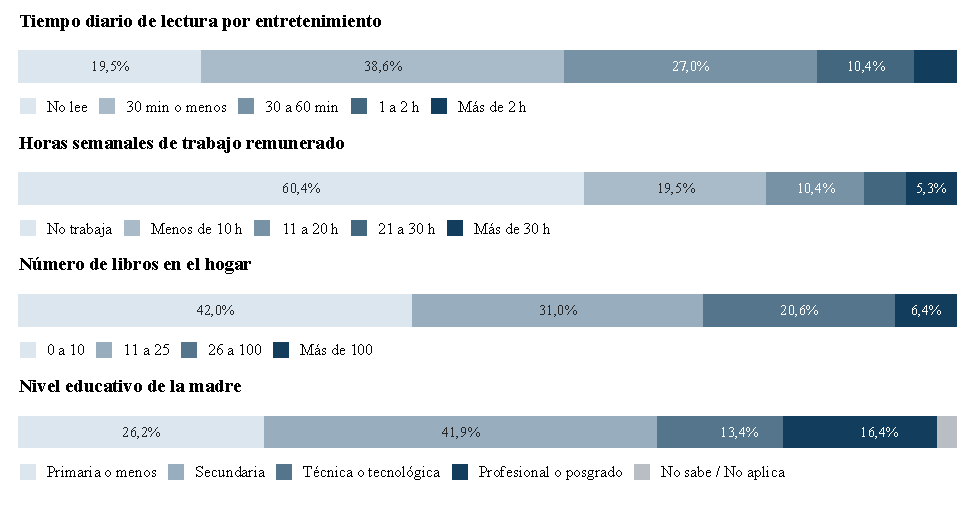
\includegraphics[width=\linewidth]{fig-ordinales}
  \end{minipage}\hfill
  \begin{minipage}[c]{0.4\textwidth}
    \captionsetup{justification=raggedright,singlelinecheck=false,skip=0pt}
    \caption{Distribución de las variables ordinales del estudiante y del hogar. La educación de
    la madre se agrupa en cuatro niveles para la figura.}
    \label{fig:ordinales}
  \end{minipage}
\end{figure}

La Figura~\ref{fig:ordinales} muestra un acceso limitado a libros y poco tiempo de lectura.
El 42{,}0\,\% de los hogares tiene diez libros o menos y el 58{,}2\,\% de los estudiantes
lee como máximo media hora diaria por entretenimiento. La educación materna se concentra
en secundaria (41{,}9\,\%) y la mayoría no trabaja (60{,}4\,\%), aunque el 9{,}8\,\%
trabaja más de veinte horas semanales. Predominan las mujeres (54{,}8\,\%) y la jornada
más frecuente es la de la mañana (39{,}7\,\%). Bogotá y Antioquia reúnen el 29{,}4\,\%
de los evaluados. Des esta manera, la baja representación de otros departamentos motiva agruparlos por
regiones en el análisis multivariado.

\FloatBarrier
\subsection{Variables cuantitativas}

\tabla{tbl-resumen-cuant}

\begin{figure}[H]
  \centering
  \begin{minipage}[c]{0.5\textwidth}
    \centering
    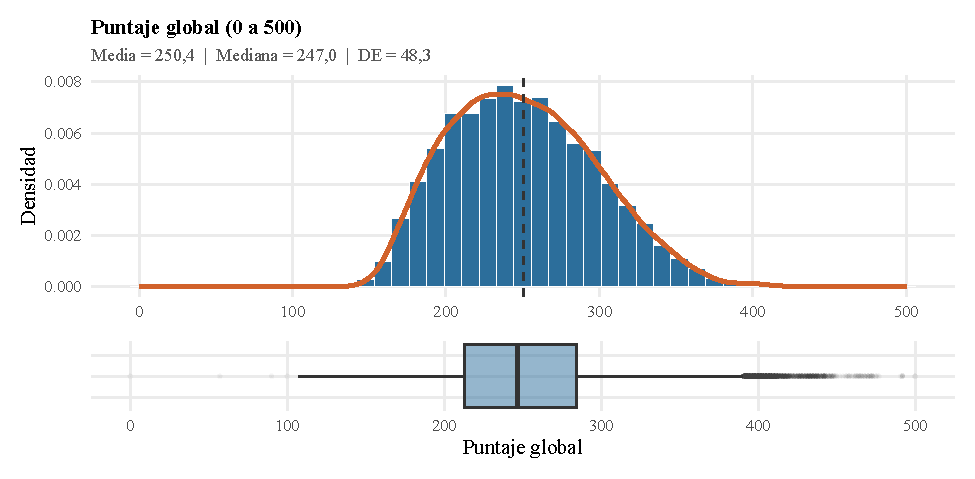
\includegraphics[width=\linewidth]{fig-global}
  \end{minipage}\hfill
  \begin{minipage}[c]{0.4\textwidth}
    \captionsetup{justification=raggedright,singlelinecheck=false,skip=0pt}
    \caption{Distribución del puntaje global: histograma con curva de densidad y diagrama de caja.}
    \label{fig:global}
  \end{minipage}
\end{figure}

El puntaje global (Tabla~\ref{tab:resumen-cuant} y Figura~\ref{fig:global}) tiene una
distribución unimodal con una leve asimetría positiva (0{,}36). La media, de 249{,}2 puntos,
supera ligeramente a la mediana, de 246{,}0, y el 50\,\% central se ubica entre 212 y 283
puntos, con una desviación estándar de 48{,}4.

\begin{figure}[H]
  \centering
  \begin{minipage}[c]{0.5\textwidth}
    \centering
    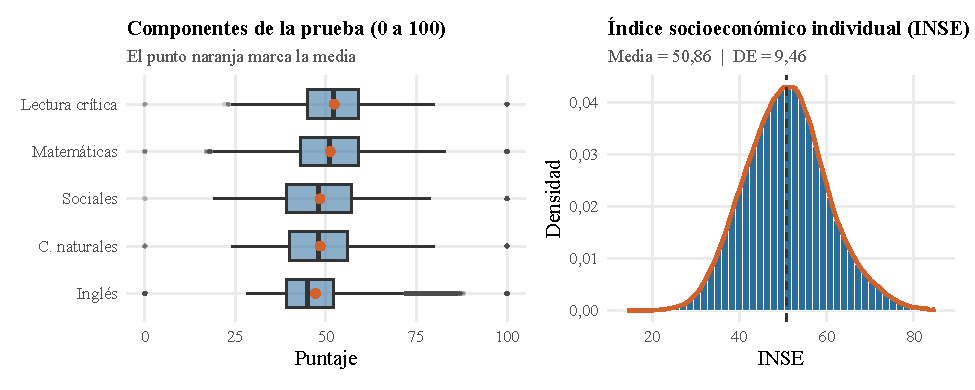
\includegraphics[width=\linewidth]{fig-componentes-inse}
  \end{minipage}\hfill
  \begin{minipage}[c]{0.4\textwidth}
    \captionsetup{justification=raggedright,singlelinecheck=false,skip=0pt}
    \caption{Puntajes de los cinco componentes en la misma escala (izquierda) y distribución del
    índice socioeconómico individual (derecha).}
    \label{fig:componentes-inse}
  \end{minipage}
\end{figure}

En la escala común de 0 a 100 (Figura~\ref{fig:componentes-inse}), Lectura Crítica
presenta la mayor media (52{,}3) y la menor dispersión relativa (CV de 19{,}3\,\%),
mientras que Sociales y Ciudadanas tiene el mayor CV (24{,}7\,\%). Inglés registra
la menor media (47{,}1) y una cola de puntajes altos (asimetría de 1{,}04).
El índice socioeconómico es casi simétrico, con media de 50{,}86 y desviación estándar
de 9{,}46. La edad, en cambio, es muy asimétrica (8{,}25): el 50\,\% central se sitúa
entre 16{,}9 y 18{,}2 años y el 1\,\% supera los 29. Por ello, la mediana (17{,}4)
representa mejor al estudiante típico que la media (17{,}9).

\FloatBarrier
\section{Análisis descriptivo bivariado}
\label{sec:bivariado}

Entre variables cuantitativas se usa el coeficiente $r$ de Pearson, cuyo cuadrado $r^2$ es la
proporción de varianza compartida. Entre una cualitativa y una cuantitativa se usa $\eta^2$, la
proporción de la varianza del puntaje que corresponde a diferencias entre las medias de los
grupos, y entre cualitativas la $V$ de Cramér, que va de 0 (independencia) a 1 (asociación
máxima). Ninguna de estas medidas implica causalidad.

\subsection{Relaciones entre variables cuantitativas}

\begin{figure}[H]
  \centering
  \begin{minipage}[c]{0.5\textwidth}
    \centering
    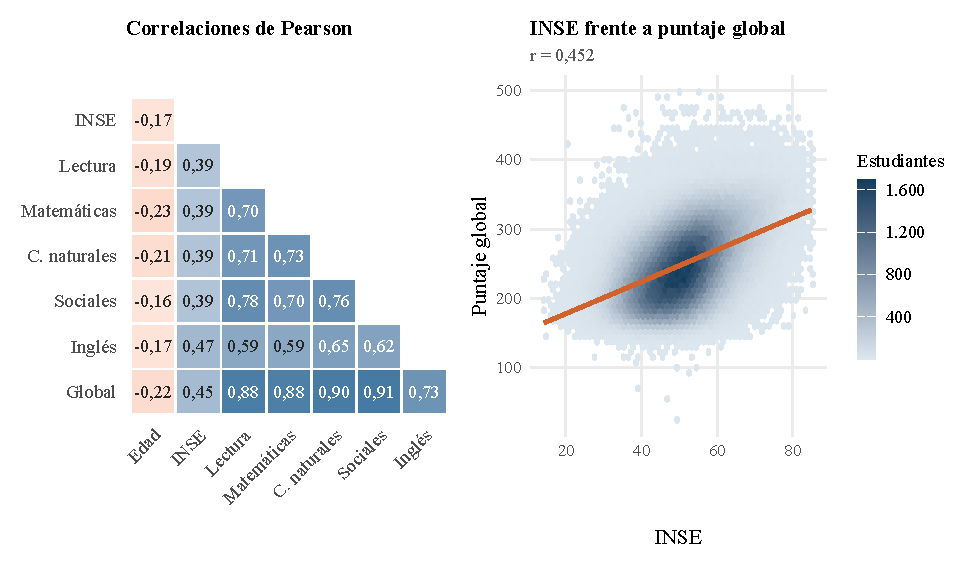
\includegraphics[width=\linewidth]{fig-corr-inse}
  \end{minipage}\hfill
  \begin{minipage}[c]{0.4\textwidth}
    \captionsetup{justification=raggedright,singlelinecheck=false,skip=0pt}
    \caption{Correlaciones de Pearson entre cuantitativas y relación
    entre el índice socioeconómico individual y el puntaje global.}
    \label{fig:corr-inse}
  \end{minipage}
\end{figure}

Los componentes presentan correlaciones de 0{,}59 a 0{,}78 (Figura~\ref{fig:corr-inse}),
mayores entre Lectura Crítica y Sociales y menores con Inglés, lo que respalda su análisis
multivariado. El índice socioeconómico se asocia moderadamente con el puntaje global
($r = 0{,}452$; 20{,}4\,\% de varianza compartida) y más con Inglés (0{,}47) que con las
demás pruebas (0{,}39). La asociación de la edad con el puntaje global es débil y negativa
($r = -0{,}22$).

\subsection{Relaciones entre las variables cualitativas y el desempeño}

\begin{figure}[H]
  \centering
  \begin{minipage}[c]{0.5\textwidth}
    \centering
    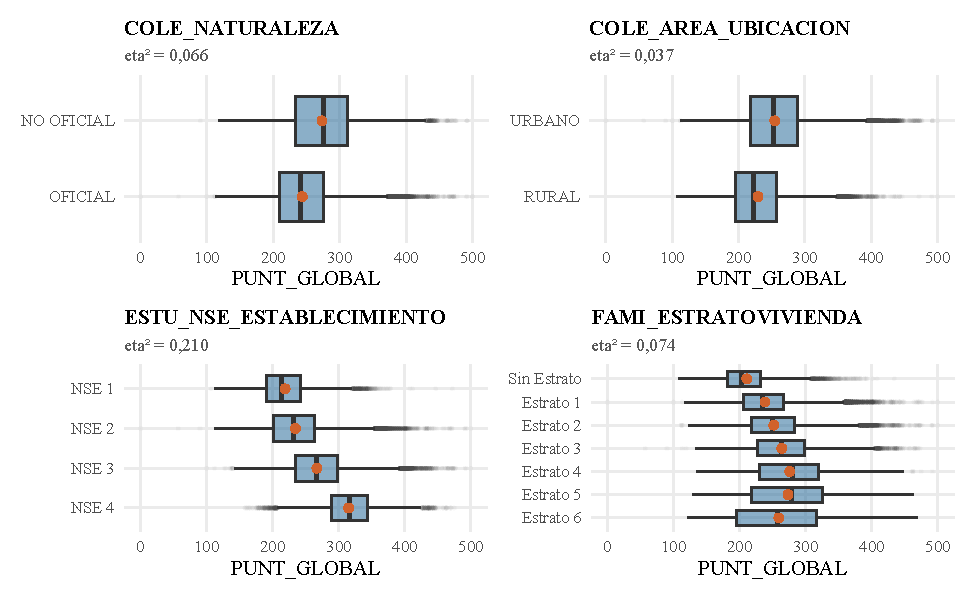
\includegraphics[width=\linewidth]{fig-box-clave}
  \end{minipage}\hfill
  \begin{minipage}[c]{0.4\textwidth}
    \captionsetup{justification=raggedright,singlelinecheck=false,skip=0pt}
    \caption{Puntaje global según el nivel socioeconómico, la naturaleza y la zona del colegio y
    la educación de la madre. El punto naranja marca la media de cada grupo.}
    \label{fig:box-clave}
  \end{minipage}
\end{figure}

\tabla{tab-asociacion}

Con una desviación estándar de 48{,}4 puntos, una brecha de 30 equivale a unas 0{,}6
desviaciones. La Figura~\ref{fig:box-clave} muestra diferencias importantes: los colegios
no oficiales promedian 271{,}9 puntos frente a 242{,}6 de los oficiales, y los urbanos,
253{,}3 frente a 228{,}0 de los rurales. La mayor brecha corresponde al NSE del colegio
(217{,}9 en NSE 1 frente a 314{,}8 en NSE 4), y por educación materna, la media es 279{,}3
con estudios profesionales o de posgrado y 228{,}8 con primaria o menos.

La Tabla~\ref{tab:asociacion} compara todas las variables por prueba. En los primeros lugares se encuentra la asociación
con el puntaje global el NSE del colegio (21{,}1\,\%), el índice socioeconómico individual
(20{,}4\,\%) y la educación materna (14{,}2\,\%), mientras que lectura (2{,}5\,\%) y género
(0{,}5\,\%) quedan entre las menores. Las asociaciones socioeconómicas son mayores en Inglés:
el NSE del colegio alcanza el 24{,}4\,\% y su naturaleza el 9{,}4\,\% (frente al
4{,}3--5{,}1\,\% de esta última en las demás pruebas). El género, de asociación casi nula
con el puntaje global y Lectura Crítica, alcanza su máximo en Matemáticas (1{,}6\,\%),
donde la edad también se asocia más. Estos contrastes justifican analizar el desempeño
por áreas, no solo mediante el puntaje global.

\subsection{Relaciones entre variables cualitativas}

\begin{figure}[H]
  \centering
  \begin{minipage}[c]{0.5\textwidth}
    \centering
    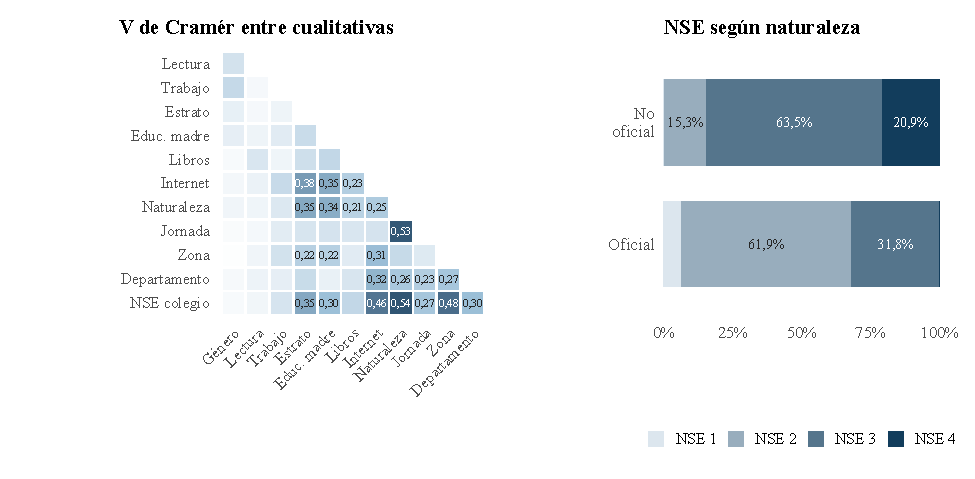
\includegraphics[width=\linewidth]{fig-cramer-nse}
  \end{minipage}\hfill
  \begin{minipage}[c]{0.4\textwidth}
    \captionsetup{justification=raggedright,singlelinecheck=false,skip=0pt}
    \caption{$V$ de Cramér entre las variables cualitativas, con valores rotulados a partir de
    0{,}20 (izquierda), y composición del nivel socioeconómico del colegio según su naturaleza
    (derecha).}
    \label{fig:cramer-nse}
  \end{minipage}
\end{figure}

Las asociaciones más fuertes se concentran en el bloque socioeconómico e institucional
(Figura~\ref{fig:cramer-nse}). El nivel socioeconómico del colegio se asocia con su naturaleza
($V = 0{,}54$), su zona (0{,}48) y el acceso a internet del hogar (0{,}46); la naturaleza, a su
vez, con la jornada (0{,}53), y el estrato con el acceso a internet (0{,}38). Las barras apiladas
muestran el par más asociado: el 20{,}9\,\% de los estudiantes de colegios no oficiales está en
NSE 4, nivel que prácticamente no existe entre los oficiales, donde el 61{,}9\,\% está en NSE 2.
En cambio, el género, la lectura y el trabajo no superan $V = 0{,}20$ con ninguna otra variable,
por lo que aportan información distinta a la del contexto socioeconómico.

Esta superposición explica por qué la suma de los porcentajes de la Tabla~\ref{tab:asociacion}
supera el 100\,\%: buena parte de lo que cada variable comparte con el puntaje es común a varias
de ellas. Separar la asociación propia de cada una exige examinarlas de manera conjunta, que es
el propósito de la técnica multivariada de la Entrega 3.

\FloatBarrier
\section{Interpretación de resultados}

\corr{En general toca volver a hacer la interpretación de resultados.}

%
% El enunciado pide analizar los resultados desde el contexto del problema de
% investigación, respondiendo preguntas como:
%   - ¿Qué comportamiento presenta la variable?
%   - ¿Existen diferencias importantes entre grupos?
%   - ¿Se observan asociaciones entre variables?
%   - ¿Qué hallazgos podrían ser relevantes para responder la pregunta de investigación?
%
% Insumos: las tablas de frecuencia y la tabla de medidas de resumen del análisis
% univariado; los diagramas de caja con eta cuadrado de la sección 11.2; la tabla de
% contingencia y la V de Cramér de la 11.3; y el ordenamiento de tamaños de efecto
% de la sección \ref{sec:efectos}. Las cifras de todas las variables, incluidas las
% que no tienen figura en este documento, están en reports/latex_entrega_2/cifras.txt.

A continuación se interpretan los resultados del análisis exploratorio a la luz de la
pregunta de investigación, donde se tendrán en cuenta los siguientes indicadores: el
comportamiento individual de las variables, las diferencias entre grupos, las asociaciones
detectadas y su lectura conjunta a partir del ordenamiento de tamaños de efecto.
 
\subsection{Comportamiento de las variables}
 
En cuanto al análisis univariado, éste deja ver que la población evaluada enfrenta,
en promedio, condiciones de vulnerabilidad considerables. Casi tres de cada diez (30\%)
hogares no cuentan con internet y cerca de cuatro de cada diez (40\%) no tienen computador,
justo en el semestre en que la educación se trasladó al hogar por la pandemia. A esto se
suma una alta concentración en los estratos bajos (90{,}1\,\% de los estudiantes en estratos 1 a 3)
y un capital educativo parental centrado en la secundaria, más bajo y peor conocido
en el caso del padre que de la madre. En el plano institucional, el sistema evaluado
es mayoritariamente oficial y urbano, con una fuerte concentración de colegios en los
niveles socioeconómicos intermedios (NSE 2 y 3). Estas cifras confirman que las variables
familiares e institucionales seleccionadas capturan una desigualdad estructural presente
en una parte considerable de la población, lo cual es un requisito necesario para que
dichas variables puedan explicar diferencias en el desempeño.
 
\subsection{Diferencias entre grupos}
 
Las comparaciones de la Sección~\ref{sec:bivariado} muestran que el desempeño académico
sí varía significativamente según el contexto del estudiante. Las brechas más grandes
están asociadas al colegio y no al estudiante persé: la diferencia entre colegios no
oficiales y oficiales es de cerca de 30 puntos, similar a la que separa a colegios
urbanos de rurales, y equivale a poco más de media desviación estándar del puntaje
global. El nivel socioeconómico del establecimiento resulta ser, de hecho, la variable
con mayor capacidad para diferenciar grupos en todo el estudio ($\eta^2 = 0{,}210$),
por encima del estrato de la vivienda del propio estudiante. Esto sugiere que el ambiente
socioeconómico compartido por los compañeros de colegio se asocia más fuertemente con el
desempeño que la condición individual del hogar. Adicionalmente, contrastando lo anterior,
se ve que variables como el género muestran diferencias pequeñas en el puntaje global
($\eta^2 = 0{,}005$), aunque no despreciables en componentes específicos como matemáticas,
lo que respalda la decisión de analizar los puntajes por área y no solo el puntaje global.
 
\subsection{Asociaciones entre variables}
 
El análisis de asociaciones evidencia que las condiciones de desventaja no actúan de
manera aislada, sino que tienden a presentarse juntas. La relación entre el estrato de
la vivienda y el acceso a internet es fuerte ($V = 0{,}382$), y la asociación más intensa
de todo el bloque cualitativo es la que existe entre la naturaleza del colegio (oficial o
no oficial) y su nivel socioeconómico ($V = 0{,}544$), lo que indica que ambas variables
describen en buena parte el mismo fenómeno visto desde dos ángulos distintos. En el plano
cuantitativo, el índice socioeconómico individual calculado por el ICFES muestra una
asociación moderada con el puntaje global ($r = 0{,}452$), consistente con la idea
de que el contexto socioeconómico influye en el desempeño sin determinarlo por
completo: existen estudiantes de bajos recursos con puntajes altos y viceversa.
Estos hallazgos son importantes porque anticipan un problema que debe resolverse
en la siguiente entrega: si las variables explicativas están correlacionadas entre
sí, no es posible sumar sus efectos individuales sin incurrir en redundancia,
lo que justifica recurrir a una técnica multivariada capaz de resumir esta estructura
compartida en unos pocos ejes (Los métodos más apropiados podrían ser PCA para cuantitativas y
MCA para cualitativas).
 
\subsection{Hallazgos relevantes para la pregunta de investigación}
 
El ordenamiento de tamaños de efecto de la \corr{Toca cambiar eso fijo} sintetiza el
hallazgo central de esta fase exploratoria: ninguna variable, por sí sola, explica
más de una quinta parte de la varianza del puntaje global. El nivel socioeconómico
del establecimiento (20{,}96\,\%) y el índice socioeconómico individual (20{,}42\,\%)
encabezan la lista, seguidos de cerca por la educación de la madre (14{,}15\,\%)
y la del padre (12{,}57\,\%), todas ellas por encima de cualquier característica
puramente individual del estudiante. Llama la atención que variables materiales simples,
como tener computador (9{,}86\,\%) o internet (9{,}16\,\%) en el hogar, recuperen una
proporción de varianza comparable e incluso mayor a la del estrato de la vivienda
(7{,}36\,\%), pese a ser indicadores binarios y no índices compuestos. En conjunto,
esta evidencia responde parcialmente a la pregunta de investigación: el desempeño
en las pruebas Saber 11 2020-2 no depende de un factor dominante, sino de la
acumulación de varias condiciones socioeconómicas, familiares e institucionales
que están parcialmente solapadas entre sí. Esto confirma la pertinencia del
enfoque multivariado planteado en los objetivos del proyecto, ya que solo una
técnica que considere el conjunto de variables de manera conjunta permitirá
establecer cuáles de ellas conservan una asociación relevante con el desempeño
una vez controladas las demás.

\section{Conclusiones del análisis exploratorio}

% Entre tres y cinco conclusiones derivadas del análisis descriptivo y exploratorio,
% que sinteticen los principales hallazgos y evidencien cómo contribuyen a comprender
% el problema de investigación.
%
% En esta etapa no se espera responder la pregunta de investigación, sino identificar
% patrones que sirvan de base para la aplicación de las técnicas de estadística
% multivariada en la Entrega 3.

\newpage

\section{Declaración de uso de inteligencia artificial}
Se usaron herramientas de Inteligencia Artificial (IA) para el desarrollo de esta entrega, para fines como mejorar la redacción, 
depurar código, automatizar cosas como exportar tablas y figuras a \LaTeX, manejo de pipelines, definir estilos para mantener consistencia,
documentación sobre el uso de herramientas como Quarto y R, y replantear enfoques o decisiones posiblemente erroneas.
En general se buscó con estas herramientas elevar la calidad del trabajo, manteniendo estructuralmente el criterio personal.

Entre las herramientas utilizadas se encuentran:
\begin{itemize}
  \item Claude (Opus 5)
  \item Prism
\end{itemize}

\section{Variables seleccionadas}
\label{anexo:variables}

\newcolumntype{L}[1]{>{\raggedright\arraybackslash}p{#1}}
\begin{longtable}{L{2.2cm} L{6.5cm} L{6.3cm}}
  \caption{Descripción de las variables seleccionadas para el análisis.}\label{tab:variables}\\
  \toprule
  \textbf{Categoría} & \textbf{Variable} & \textbf{Descripción} \\
  \midrule
  \endfirsthead

  \midrule
  \multicolumn{3}{r}{\textit{Continúa en la página siguiente...}} \\
  \midrule
  \textbf{Categoría} & \textbf{Variable} & \textbf{Descripción} \\
  \midrule
  \endhead

  \midrule
  \multicolumn{3}{r}{\textit{Continúa en la página siguiente...}} \\
  \endfoot

  \bottomrule
  \endlastfoot

  % --- Características demográficas ---
  \midrule
  \multicolumn{3}{l}{\textit{Características demográficas}} \\
  ESTU & \texttt{ESTU\_GENERO} & Género reportado por el estudiante. \\
  ESTU & \texttt{ESTU\_FECHANACIMIENTO} & Fecha de nacimiento; se utiliza para calcular la edad al momento de presentar la prueba. \\

    % --- Hábitos y dedicación ---
  \midrule
  \multicolumn{3}{l}{\textit{Hábitos y dedicación}} \\
  ESTU & \texttt{ESTU\_DEDICACIONLECTURADIARIA} & Tiempo diario dedicado a la lectura fuera del ámbito escolar. \\
  ESTU & \texttt{ESTU\_HORASSEMANATRABAJA} & Número de horas semanales dedicadas a trabajo remunerado. \\

  % --- Condiciones del hogar ---
  \midrule
  \multicolumn{3}{l}{\textit{Condiciones del hogar}} \\
  FAMI & \texttt{FAMI\_ESTRATOVIVIENDA} & Estrato socioeconómico de la vivienda (1 a 6, según clasificación del DANE). \\

  % --- Capital educativo y cultural del hogar ---
  \midrule
  \multicolumn{3}{l}{\textit{Capital educativo y cultural del hogar}} \\
  FAMI & \texttt{FAMI\_EDUCACIONMADRE} & Nivel educativo máximo alcanzado por la madre o figura materna (ordinal). \\
  FAMI & \texttt{FAMI\_NUMLIBROS} & Cantidad aproximada de libros presentes en el hogar (ordinal). \\

  % --- Acceso tecnológico ---
  \midrule
  \multicolumn{3}{l}{\textit{Acceso tecnológico}} \\
  FAMI & \texttt{FAMI\_TIENEINTERNET} & Indica si el hogar cuenta con servicio de internet. \\

  % --- Establecimiento educativo ---
  \midrule
  \multicolumn{3}{l}{\textit{Características del establecimiento educativo}} \\
  COLE & \texttt{COLE\_NATURALEZA} & Naturaleza jurídica del colegio (oficial o no oficial). \\
  COLE & \texttt{COLE\_JORNADA} & Jornada en la que funciona el colegio (mañana, tarde, noche, única, completa, sabatina). \\
  COLE & \texttt{COLE\_AREA\_UBICACION} & Área de ubicación del colegio (urbana o rural). \\
  COLE & \texttt{COLE\_DEPTO\_UBICACION} & Departamento donde se encuentra ubicado el colegio. \\

  % --- Índices socioeconómicos ---
  \midrule
  \multicolumn{3}{l}{\textit{Índices socioeconómicos}} \\
  ESTU & \texttt{ESTU\_INSE\_INDIVIDUAL} & Índice socioeconómico individual calculado por el ICFES (continuo). \\
  ESTU & \texttt{ESTU\_NSE\_ESTABLECIMIENTO} & Nivel socioeconómico promedio del establecimiento educativo (ordinal). \\

  % --- Desempeño académico ---
  \midrule
  \multicolumn{3}{l}{\textit{Desempeño académico (variables de respuesta)}} \\
  PUNT & \texttt{PUNT\_LECTURA\_CRITICA} & Puntaje obtenido en la prueba de lectura crítica (0--100). \\
  PUNT & \texttt{PUNT\_MATEMATICAS} & Puntaje obtenido en la prueba de matemáticas (0--100). \\
  PUNT & \texttt{PUNT\_C\_NATURALES} & Puntaje obtenido en la prueba de ciencias naturales (0--100). \\
  PUNT & \texttt{PUNT\_SOCIALES\_CIUDADANAS} & Puntaje obtenido en la prueba de sociales y ciudadanas (0--100). \\
  PUNT & \texttt{PUNT\_INGLES} & Puntaje obtenido en la prueba de inglés (0--100). \\
  PUNT & \texttt{PUNT\_GLOBAL} & Puntaje global del estudiante, calculado como promedio ponderado de las cinco pruebas. \\

  % --- Criterio de filtro ---
  \midrule
  \multicolumn{3}{l}{\textit{Criterio de filtro}} \\
  ESTU & \texttt{ESTU\_ESTADOINVESTIGACION} & Estado del registro dentro del proceso de investigación del ICFES; se
  conservan únicamente los registros publicables. \\
\end{longtable}

\printbibliography[title={Referencias}]

\end{document}